% Generated by Sphinx.
\def\sphinxdocclass{report}
\documentclass[letterpaper,10pt,english]{sphinxmanual}

        \usepackage{ucs}
        \usepackage[utf8x]{inputenc}

\usepackage[T1]{fontenc}
\usepackage{babel}
\usepackage{times}
\usepackage[Bjarne]{fncychap}
\usepackage{longtable}
\usepackage{sphinx}
\usepackage{multirow}

    \usepackage{wrapfig}
    \usepackage{caption}
    \captionsetup{justification=raggedleft,singlelinecheck=false}

\title{Moderation Documentation}
\date{March 09, 2012}
\release{7.x-1.x-dev}
\author{Melissa Anderson \textless{}eliza411\textgreater{}}
\newcommand{\sphinxlogo}{
\includegraphics{opensourcery.png}\par}
\renewcommand{\releasename}{Release}
\makeindex

\makeatletter
\def\PYG@reset{\let\PYG@it=\relax \let\PYG@bf=\relax%
    \let\PYG@ul=\relax \let\PYG@tc=\relax%
    \let\PYG@bc=\relax \let\PYG@ff=\relax}
\def\PYG@tok#1{\csname PYG@tok@#1\endcsname}
\def\PYG@toks#1+{\ifx\relax#1\empty\else%
    \PYG@tok{#1}\expandafter\PYG@toks\fi}
\def\PYG@do#1{\PYG@bc{\PYG@tc{\PYG@ul{%
    \PYG@it{\PYG@bf{\PYG@ff{#1}}}}}}}
\def\PYG#1#2{\PYG@reset\PYG@toks#1+\relax+\PYG@do{#2}}

\def\PYG@tok@gd{\def\PYG@tc##1{\textcolor[rgb]{0.63,0.00,0.00}{##1}}}
\def\PYG@tok@gu{\let\PYG@bf=\textbf\def\PYG@tc##1{\textcolor[rgb]{0.50,0.00,0.50}{##1}}}
\def\PYG@tok@gt{\def\PYG@tc##1{\textcolor[rgb]{0.00,0.25,0.82}{##1}}}
\def\PYG@tok@gs{\let\PYG@bf=\textbf}
\def\PYG@tok@gr{\def\PYG@tc##1{\textcolor[rgb]{1.00,0.00,0.00}{##1}}}
\def\PYG@tok@cm{\let\PYG@it=\textit\def\PYG@tc##1{\textcolor[rgb]{0.25,0.50,0.56}{##1}}}
\def\PYG@tok@vg{\def\PYG@tc##1{\textcolor[rgb]{0.73,0.38,0.84}{##1}}}
\def\PYG@tok@m{\def\PYG@tc##1{\textcolor[rgb]{0.13,0.50,0.31}{##1}}}
\def\PYG@tok@mh{\def\PYG@tc##1{\textcolor[rgb]{0.13,0.50,0.31}{##1}}}
\def\PYG@tok@cs{\def\PYG@tc##1{\textcolor[rgb]{0.25,0.50,0.56}{##1}}\def\PYG@bc##1{\colorbox[rgb]{1.00,0.94,0.94}{##1}}}
\def\PYG@tok@ge{\let\PYG@it=\textit}
\def\PYG@tok@vc{\def\PYG@tc##1{\textcolor[rgb]{0.73,0.38,0.84}{##1}}}
\def\PYG@tok@il{\def\PYG@tc##1{\textcolor[rgb]{0.13,0.50,0.31}{##1}}}
\def\PYG@tok@go{\def\PYG@tc##1{\textcolor[rgb]{0.19,0.19,0.19}{##1}}}
\def\PYG@tok@cp{\def\PYG@tc##1{\textcolor[rgb]{0.00,0.44,0.13}{##1}}}
\def\PYG@tok@gi{\def\PYG@tc##1{\textcolor[rgb]{0.00,0.63,0.00}{##1}}}
\def\PYG@tok@gh{\let\PYG@bf=\textbf\def\PYG@tc##1{\textcolor[rgb]{0.00,0.00,0.50}{##1}}}
\def\PYG@tok@ni{\let\PYG@bf=\textbf\def\PYG@tc##1{\textcolor[rgb]{0.84,0.33,0.22}{##1}}}
\def\PYG@tok@nl{\let\PYG@bf=\textbf\def\PYG@tc##1{\textcolor[rgb]{0.00,0.13,0.44}{##1}}}
\def\PYG@tok@nn{\let\PYG@bf=\textbf\def\PYG@tc##1{\textcolor[rgb]{0.05,0.52,0.71}{##1}}}
\def\PYG@tok@no{\def\PYG@tc##1{\textcolor[rgb]{0.38,0.68,0.84}{##1}}}
\def\PYG@tok@na{\def\PYG@tc##1{\textcolor[rgb]{0.25,0.44,0.63}{##1}}}
\def\PYG@tok@nb{\def\PYG@tc##1{\textcolor[rgb]{0.00,0.44,0.13}{##1}}}
\def\PYG@tok@nc{\let\PYG@bf=\textbf\def\PYG@tc##1{\textcolor[rgb]{0.05,0.52,0.71}{##1}}}
\def\PYG@tok@nd{\let\PYG@bf=\textbf\def\PYG@tc##1{\textcolor[rgb]{0.33,0.33,0.33}{##1}}}
\def\PYG@tok@ne{\def\PYG@tc##1{\textcolor[rgb]{0.00,0.44,0.13}{##1}}}
\def\PYG@tok@nf{\def\PYG@tc##1{\textcolor[rgb]{0.02,0.16,0.49}{##1}}}
\def\PYG@tok@si{\let\PYG@it=\textit\def\PYG@tc##1{\textcolor[rgb]{0.44,0.63,0.82}{##1}}}
\def\PYG@tok@s2{\def\PYG@tc##1{\textcolor[rgb]{0.25,0.44,0.63}{##1}}}
\def\PYG@tok@vi{\def\PYG@tc##1{\textcolor[rgb]{0.73,0.38,0.84}{##1}}}
\def\PYG@tok@nt{\let\PYG@bf=\textbf\def\PYG@tc##1{\textcolor[rgb]{0.02,0.16,0.45}{##1}}}
\def\PYG@tok@nv{\def\PYG@tc##1{\textcolor[rgb]{0.73,0.38,0.84}{##1}}}
\def\PYG@tok@s1{\def\PYG@tc##1{\textcolor[rgb]{0.25,0.44,0.63}{##1}}}
\def\PYG@tok@gp{\let\PYG@bf=\textbf\def\PYG@tc##1{\textcolor[rgb]{0.78,0.36,0.04}{##1}}}
\def\PYG@tok@sh{\def\PYG@tc##1{\textcolor[rgb]{0.25,0.44,0.63}{##1}}}
\def\PYG@tok@ow{\let\PYG@bf=\textbf\def\PYG@tc##1{\textcolor[rgb]{0.00,0.44,0.13}{##1}}}
\def\PYG@tok@sx{\def\PYG@tc##1{\textcolor[rgb]{0.78,0.36,0.04}{##1}}}
\def\PYG@tok@bp{\def\PYG@tc##1{\textcolor[rgb]{0.00,0.44,0.13}{##1}}}
\def\PYG@tok@c1{\let\PYG@it=\textit\def\PYG@tc##1{\textcolor[rgb]{0.25,0.50,0.56}{##1}}}
\def\PYG@tok@kc{\let\PYG@bf=\textbf\def\PYG@tc##1{\textcolor[rgb]{0.00,0.44,0.13}{##1}}}
\def\PYG@tok@c{\let\PYG@it=\textit\def\PYG@tc##1{\textcolor[rgb]{0.25,0.50,0.56}{##1}}}
\def\PYG@tok@mf{\def\PYG@tc##1{\textcolor[rgb]{0.13,0.50,0.31}{##1}}}
\def\PYG@tok@err{\def\PYG@bc##1{\fcolorbox[rgb]{1.00,0.00,0.00}{1,1,1}{##1}}}
\def\PYG@tok@kd{\let\PYG@bf=\textbf\def\PYG@tc##1{\textcolor[rgb]{0.00,0.44,0.13}{##1}}}
\def\PYG@tok@ss{\def\PYG@tc##1{\textcolor[rgb]{0.32,0.47,0.09}{##1}}}
\def\PYG@tok@sr{\def\PYG@tc##1{\textcolor[rgb]{0.14,0.33,0.53}{##1}}}
\def\PYG@tok@mo{\def\PYG@tc##1{\textcolor[rgb]{0.13,0.50,0.31}{##1}}}
\def\PYG@tok@mi{\def\PYG@tc##1{\textcolor[rgb]{0.13,0.50,0.31}{##1}}}
\def\PYG@tok@kn{\let\PYG@bf=\textbf\def\PYG@tc##1{\textcolor[rgb]{0.00,0.44,0.13}{##1}}}
\def\PYG@tok@o{\def\PYG@tc##1{\textcolor[rgb]{0.40,0.40,0.40}{##1}}}
\def\PYG@tok@kr{\let\PYG@bf=\textbf\def\PYG@tc##1{\textcolor[rgb]{0.00,0.44,0.13}{##1}}}
\def\PYG@tok@s{\def\PYG@tc##1{\textcolor[rgb]{0.25,0.44,0.63}{##1}}}
\def\PYG@tok@kp{\def\PYG@tc##1{\textcolor[rgb]{0.00,0.44,0.13}{##1}}}
\def\PYG@tok@w{\def\PYG@tc##1{\textcolor[rgb]{0.73,0.73,0.73}{##1}}}
\def\PYG@tok@kt{\def\PYG@tc##1{\textcolor[rgb]{0.56,0.13,0.00}{##1}}}
\def\PYG@tok@sc{\def\PYG@tc##1{\textcolor[rgb]{0.25,0.44,0.63}{##1}}}
\def\PYG@tok@sb{\def\PYG@tc##1{\textcolor[rgb]{0.25,0.44,0.63}{##1}}}
\def\PYG@tok@k{\let\PYG@bf=\textbf\def\PYG@tc##1{\textcolor[rgb]{0.00,0.44,0.13}{##1}}}
\def\PYG@tok@se{\let\PYG@bf=\textbf\def\PYG@tc##1{\textcolor[rgb]{0.25,0.44,0.63}{##1}}}
\def\PYG@tok@sd{\let\PYG@it=\textit\def\PYG@tc##1{\textcolor[rgb]{0.25,0.44,0.63}{##1}}}

\def\PYGZbs{\char`\\}
\def\PYGZus{\char`\_}
\def\PYGZob{\char`\{}
\def\PYGZcb{\char`\}}
\def\PYGZca{\char`\^}
\def\PYGZsh{\char`\#}
\def\PYGZpc{\char`\%}
\def\PYGZdl{\char`\$}
\def\PYGZti{\char`\~}
% for compatibility with earlier versions
\def\PYGZat{@}
\def\PYGZlb{[}
\def\PYGZrb{]}
\makeatother

\begin{document}

\maketitle
\tableofcontents
\phantomsection\label{index::doc}


Contents:

Does your organization require content review before the content gets published? We'll build a common editorial workflow that allows an author to create and edit his or her own work and submit it for editorial review. Author and editor can collaborate until it's ready to be passed along for final approval and publication.
\begin{figure}[htbp]
\centering
\capstart


\includegraphics{sites/default/files/recipes/user_icons/contributor.png}
\caption{Cathy Contributor}{\small 
Cathy has been assigned the Contributor role so that she will be able to create and edit her own content.
}\end{figure}
\begin{figure}[htbp]
\centering
\capstart


\includegraphics{sites/default/files/recipes/user_icons/editor.png}
\caption{Eli Editor}{\small 
Eli has been assigned the Editor role so that in addition to being able to do anything a contributor can do, he will be able to edit the work of others and advance content for publication.
}\end{figure}
\begin{figure}[htbp]
\centering
\capstart


\includegraphics{sites/default/files/recipes/user_icons/publisher.png}
\caption{Peggy Publisher}{\small 
Peggy has been assigned the Publisher role. This is the only role that will be able to make content live on the site. Publishers can do everything that editors and contributors can do.
}\end{figure}


\chapter{Ingredients}
\label{moderation:welcome-to-test-kitchen-documentation}\label{moderation::doc}\label{moderation:ingredients}
Test kitchen recipes are based on our sandbox setup, which includes pre-installed modules used every time. See \href{http://training.opensourcery.com/sandbox/setup}{http://training.opensourcery.com/sandbox/setup} to configure your own environment to match these instructions.


\section{Staple}
\label{moderation:staple}\begin{enumerate}
\item {} 
\href{http://drupal.org/project/ctools}{http://drupal.org/project/ctools} - Enable Chaos tools

\item {} 
\href{http://drupal.org/project/views}{http://drupal.org/project/views} - Enable Views and Views UI

\item {} 
\href{http://drupal.org/project/advanced\_help}{http://drupal.org/project/advanced\_help} - Enable Advanced Help

\item {} 
\href{http://drupal.org/project/workbench}{http://drupal.org/project/workbench} - Enable Workbench

\item {} 
\href{http://drupal.org/project/workbench\_moderation}{http://drupal.org/project/workbench\_moderation} - Use the development version. Enable Workbench Moderation

\item {} 
\href{http://drupal.org/project/diff}{http://drupal.org/project/diff} - Enable Diff

\end{enumerate}

\textbf{Drush users:}

\begin{Verbatim}[commandchars=\\\{\}]
drush dl ctools views workbench workbench\_moderation-7.x-1.x-dev diff
drush en ctools views views\_ui workbench workbench\_moderation diff -y
\end{Verbatim}


\chapter{Users and permissions}
\label{moderation:users-and-permissions}
\emph{People \textgreater{} Permissions}

We're working with three pre-created users, each of which is assigned to one of the three pre-created roles that will be used in the workflow. Creating users and roles is routine, but permissions are one of the trickiest things to get right, so that's where we'll begin.


\section{Node permissions}
\label{moderation:node-permissions}
Before setting up the second layer of permissions provided by Workbench Moderation, we'll set the basic node permissions. These settings are based on the premise that no site content is ever deleted. During development, you might choose to allow the deletion of content.

\begin{tabulary}{\linewidth}{|L|L|L|L|}
\hline
\textbf{
Permission
} & \textbf{
Contributor
} & \textbf{
Editor
} & \textbf{
Publisher
}\\\hline

View own unpublished content
 & 
{[}√{]}
 & 
{[}√{]}
 & 
{[}√{]}
\\\hline

View content revisions
 & 
{[}√{]}
 & 
{[}√{]}
 & 
{[}√{]}
\\\hline

Revert content revisions
 & 
{[} {]}
 & 
{[}√{]}
 & 
{[}√{]}
\\\hline

Delete content revisions
 & 
{[} {]}
 & 
{[} {]}
 & 
{[} {]}
\\\hline

Article: Create new content
 & 
{[}√{]}
 & 
{[}√{]}
 & 
{[}√{]}
\\\hline

Article: Edit own content
 & 
{[}√{]}
 & 
{[}√{]}
 & 
{[}√{]}
\\\hline

Article: Edit any content
 & 
{[} {]}
 & 
{[}√{]}
 & 
{[}√{]}
\\\hline

Article: Delete own content
 & 
{[} {]}
 & 
{[} {]}
 & 
{[} {]}
\\\hline

Article: Delete any content
 & 
{[} {]}
 & 
{[} {]}
 & 
{[} {]}
\\\hline

Basic page: Create new content
 & 
{[}√{]}
 & 
{[}√{]}
 & 
{[}√{]}
\\\hline

Basic page: Edit own content
 & 
{[}√{]}
 & 
{[}√{]}
 & 
{[}√{]}
\\\hline

Basic page: Edit any content
 & 
{[} {]}
 & 
{[}√{]}
 & 
{[}√{]}
\\\hline

Basic page: Delete own content
 & 
{[} {]}
 & 
{[} {]}
 & 
{[} {]}
\\\hline

Basic page: Delete any content
 & 
{[} {]}
 & 
{[} {]}
 & 
{[} {]}
\\\hline
\end{tabulary}



\chapter{Configure workbench moderation}
\label{moderation:configure-workbench-moderation}

\section{Review configuration}
\label{moderation:review-configuration}
\emph{Configuration \textgreater{} Workbench: Workbench Moderation}

{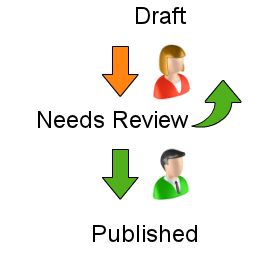
\includegraphics{sites/default/files/recipes/moderation/workflow_simple.png}\hfill}

We will start by using the default states provided by Workbench Moderation and later add new ones. These states are adequate for the simple workflow pictured here. When we add a third role for review prior to publication, then we'll need to make adjustments.


\section{Enable the workflow for content types}
\label{moderation:enable-the-workflow-for-content-types}
\emph{Structure \textgreater{} Content types \textgreater{} Article: edit}

Although we don't cover this today, it is possible to moderate content on a per-content-type basis. This gets complex very quickly! See \href{http://drupal.org/node/1206854\#comment-5241230}{http://drupal.org/node/1206854\#comment-5241230} for how to enable this.
\begin{enumerate}
\item {} 
Publishing options

\item {} 
{[} {]} Published \textless{}-Uncheck this

\item {} 
{[}√{]} Promoted to front page \textless{}- Leave checked

\item {} 
{[} {]} Sticky at top of lists \textless{}- Leave unchecked

\item {} 
{[}√{]} Create a new revision \textless{}- Check this!

\item {} 
{[}√{]} Enable moderation of revisions \textless{}- Can only be checked once the item above is checked. Check this).

\item {} 
Default moderation state: Draft

\item {} 
Save content type

\item {} 
Repeat for the Basic page content type, although don't promote pages to the front page)

\end{enumerate}


\section{Set the Workbench Moderation permissions}
\label{moderation:set-the-workbench-moderation-permissions}
\emph{People \textgreater{} Permissions}

At the bottom of the Permissions page:

\textbf{Workbench}

\begin{tabulary}{\linewidth}{|L|L|L|L|}
\hline
\textbf{
Permission
} & \textbf{
Contributor
} & \textbf{
Editor
} & \textbf{
Publisher
}\\\hline

Administer Workbench settings
 & 
{[} {]}
 & 
{[} {]}
 & 
{[} {]}
\\\hline

Access My Workbench
 & 
{[}√{]}
 & 
{[}√{]}
 & 
{[}√{]}
\\\hline
\end{tabulary}


\textbf{Workbench Moderation}

\begin{tabulary}{\linewidth}{|L|L|L|L|}
\hline
\textbf{
Permission
} & \textbf{
Contributor
} & \textbf{
Editor
} & \textbf{
Publisher
}\\\hline

View all unpublished content
 & 
{[} {]}
 & 
{[}√{]}
 & 
{[}√{]}
\\\hline

Administer Workbench Moderation
 & 
{[} {]}
 & 
{[} {]}
 & 
{[} {]}
\\\hline

Bypass moderation restrictions
 & 
{[} {]}
 & 
{[} {]}
 & 
{[} {]}
\\\hline

View moderation history
 & 
{[}√{]}
 & 
{[}√{]}
 & 
{[}√{]}
\\\hline

View the moderation messages on a node
 & 
{[}√{]}
 & 
{[}√{]}
 & 
{[}√{]}
\\\hline

Use ``My Drafts'' workbench tab
 & 
{[}√{]}
 & 
{[}√{]}
 & 
{[}√{]}
\\\hline

Use ``Needs Review'' workbench tab
 & 
{[} {]}
 & 
{[}√{]}
 & 
{[}√{]}
\\\hline

Moderate all content from Draft to Needs Review *
 & 
{[}√{]}
 & 
{[}√{]}
 & 
{[}√{]}
\\\hline

Moderate all content from  Needs Review to Draft
 & 
{[} {]}
 & 
{[}√{]}
 & 
{[}√{]}
\\\hline

Moderate all content from Needs Review to Published
 & 
{[} {]}
 & 
{[}√{]}
 & 
{[}√{]}
\\\hline
\end{tabulary}


* You must grant this permission to the Contributor. It is limited in scope by the specific node permissions for each content type. In our case, the Contributor role is only allowed to edit its own Articles and Basic Pages, so a user with that role can only move their own content from Draft to Needs review. Cathy Contributor won't be able to moderate other peoples' work.


\section{Check your permissions}
\label{moderation:check-your-permissions}
\emph{Configuration \textgreater{} Workbench: Workbench Moderation \textgreater{} Check permissions (tab)}

Workbench has a great feature to help ensure you've set up your transitions properly. Test both to be sure that each role can do what you want and also that no roles can do things they're not supposed to.


\chapter{Watch Contributor \textgreater{} Editor Moderation in Action}
\label{moderation:watch-contributor-editor-moderation-in-action}
We're going to set up in two separate browsers, one for Cathy Contributor and one for Eli Editor so that we can watch as content progresses through the workflow.


\section{Create an article as Cathy Contributor}
\label{moderation:faq}\label{moderation:create-an-article-as-cathy-contributor}
\emph{Add content \textgreater{} Article}
\begin{figure}[htbp]
\centering


\includegraphics{sites/default/files/recipes/user_icons/contributor.png}
{\small \begin{enumerate}
\item {} 
In the first browser, logged in as admin, masquerade as Cathy Contributor.

\item {} 
Create a new article titled Contributor FAQ

\item {} 
Note the message that the draft will be placed in moderation.

\end{enumerate}
}\end{figure}


\section{View Eli Editor's Worbench}
\label{moderation:view-eli-editor-s-worbench}
\emph{My Workbench \textgreater{} Needs Review (tab)}
\begin{figure}[htbp]
\centering


\includegraphics{sites/default/files/recipes/user_icons/editor.png}
{\small 
To save yourself the tedium of logging in and out or even masquerading back and forth, we recommend you install a second browser on your system, if you don't already have one.
\begin{enumerate}
\item {} 
In the second browser, logged in as admin, masquerade as Eli Editor.

\item {} 
View My Workbench \textgreater{} Needs Review (tab)

\item {} 
You shouldn't see anything yet.

\end{enumerate}
}\end{figure}


\section{Move Cathy's work to Needs Review}
\label{moderation:move-cathy-s-work-to-needs-review}
\emph{Workbench \textgreater{} My Drafts}
\begin{figure}[htbp]
\centering


\includegraphics{sites/default/files/recipes/user_icons/contributor.png}
{\small 
Cathy Contributor can move her work from Draft to Needs Review in three places:
\begin{itemize}
\item {} 
On the View draft tab of the node, just as soon as she's saved it

\item {} 
On the Moderate tab, where the entire revision history is available

\item {} 
From the My Drafts page

\end{itemize}

Her work will will enter the workflow when she moves it to the Needs Review state.
\begin{enumerate}
\item {} 
Move the article we created, Contributor FAQ, into the Needs Review state.

\end{enumerate}
\begin{enumerate}
\setcounter{enumi}{1}
\item {} 
Note that it disappears from Drafts and reappears on the My content page in My Edits. If Cathy bookmarks the page, she can still edit this while it's in the Needs review state, good for fixing that last typo.

\end{enumerate}
}\end{figure}


\section{Publish Cathy's article}
\label{moderation:publish-cathy-s-article}
\emph{My Workbench \textgreater{} Needs Review (tab)}
\begin{figure}[htbp]
\centering


\includegraphics{sites/default/files/recipes/user_icons/editor.png}
{\small \begin{enumerate}
\item {} 
Reload Eli Editor's Needs Review tab.

\item {} 
Locate Cathy's new article.

\item {} 
Publish it.

\end{enumerate}
}\end{figure}


\section{As Cathy, review the published work}
\label{moderation:as-cathy-review-the-published-work}
\emph{My Workbench}:
\begin{figure}[htbp]
\centering


\includegraphics{sites/default/files/recipes/user_icons/contributor.png}
{\small \begin{enumerate}
\item {} 
Take a look at Cathy's main workbench page.

\item {} 
Edit the Contributor FAQ

\item {} 
Note that the officially-approved content stays published while this draft goes into moderation.

\end{enumerate}
}\end{figure}


\section{Experiment}
\label{moderation:experiment}\begin{enumerate}
\item {} 
Try routing the article between Cathy and Eli in ways your organization might use workflow.

\item {} 
Try creating content as Eli.

\item {} 
Switch back to the admin account when you're done.

\end{enumerate}

What if Eli would like to return the article to Cathy because it needs work? He can send it back by setting it to Draft, but out of the box, it's difficult to add a message to the page. We'll fix that as best we can in the section {\hyperref[moderation:views]{\emph{Adjust the views}}}. There is a feature request to make it easier to add comments at \href{http://drupal.org/node/1257650}{http://drupal.org/node/1257650}.


\chapter{View the differences between revisions}
\label{moderation:view-the-differences-between-revisions}
We're working with the development version of Workbench Moderation in order to demonstrate how to highlight differences between two revisions. The dev version incorporates output from the diff module, which was installed at the beginning on the recipe.

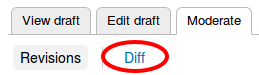
\includegraphics{sites/default/files/recipes/moderation/diff.png}
\begin{enumerate}
\item {} 
Diff \textless{}- Click the workd

\item {} 
Select a radio button in each column

\item {} 
Show Diff

You can follow plans for an improved user interface in the 2.x version at \href{http://drupal.org/node/1404642}{http://drupal.org/node/1404642}.

\end{enumerate}


\chapter{Expanding the Workflow}
\label{moderation:expanding-the-workflow}

\section{Add a new state}
\label{moderation:add-a-new-state}
\emph{Configuration \textgreater{} Workbench: Workbench Moderation}

{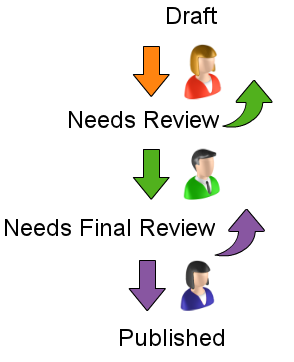
\includegraphics{sites/default/files/recipes/moderation/workflow.png}\hfill}

To add the publisher into the mix, we need a state for content that has been approved by the editor and needs a final review by the publisher.
\begin{quote}

On the main screen, add a state:
\begin{quote}
\begin{enumerate}
\item {} 
Name: Needs Final Review

\item {} 
Description: Ready for publication

\item {} 
Arrange them in order using the grabber
\begin{itemize}
\item {} 
Draft

\item {} 
Needs Review

\item {} 
Needs Final Review

\item {} 
Published

\end{itemize}

\end{enumerate}
\begin{enumerate}
\setcounter{enumi}{3}
\item {} 
Save

\end{enumerate}
\end{quote}
\end{quote}

When you save, you'll see the following warning:

Depending on the changes you have made it may be necessary to reconfigure Views that leverage Workbench Moderation such as workbench\_moderation.

The section {\hyperref[moderation:views]{\emph{Adjust the views}}} will address the customizations necessary to take advantage of our new state.


\section{Enable the transitions}
\label{moderation:enable-the-transitions}
\emph{Configuration \textgreater{} Workbench: Workbench Moderation: Transitions (tab)}

Next we define the transitions:

Allow us to give editors permission to advance content to publishers.
\begin{enumerate}
\item {} 
Needs Review \textgreater{} Needs Final Review

\item {} 
Save

\end{enumerate}

Allow us to give publishers the ability to send the content back to the editors.
\begin{enumerate}
\item {} 
Needs Final Review \textgreater{} Needs Review

\item {} 
Save

\end{enumerate}

Allow us to give the publisher permission to publish.
\begin{enumerate}
\item {} 
Needs Final Review \textgreater{} Published

\item {} 
Save

\end{enumerate}

Remove an editor's ability to publish without final review.
\begin{enumerate}
\item {} 
Needs Review \textgreater{} Published \textless{}- Check delete

\item {} 
Save

\end{enumerate}


\section{Assign transition permissions}
\label{moderation:assign-transition-permissions}
\emph{People \textgreater{} Permissions}

Set permissions for the new states as follows.

\textbf{Workbench Moderation}

\begin{tabulary}{\linewidth}{|L|L|L|L|}
\hline
\textbf{
Permission
} & \textbf{
Contributor
} & \textbf{
Editor
} & \textbf{
Publisher
}\\\hline

Moderate all content from Needs Review to Needs Final Review
 & 
{[} {]}
 & 
{[}√{]}
 & 
{[}√{]}
\\\hline

Moderate all content from Needs Final Review to Needs Review
 & 
{[} {]}
 & 
{[} {]}
 & 
{[}√{]}
\\\hline

Moderate all content from Needs Final Review to Published
 & 
{[} {]}
 & 
{[} {]}
 & 
{[}√{]}
\\\hline
\end{tabulary}



\chapter{Adjust the views}
\label{moderation:adjust-the-views}\label{moderation:views}

\section{Add an administration page for publishers}
\label{moderation:add-an-administration-page-for-publishers}
\emph{Structure \textgreater{} Views \textgreater{} workbench\_moderation: edit}


\subsection{Displays}
\label{moderation:displays}
This is a critically important step. Be sure you're working with the display you think you are!
\begin{enumerate}
\item {} 
Click Needs Review Page \textless{}- even if it's already selected I never skip this step.

\end{enumerate}


\subsection{Needs Review Page details}
\label{moderation:needs-review-page-details}\begin{enumerate}
\item {} 
Click the arrow next to `view needs review page'

\item {} 
Choose `clone needs review page'

\item {} 
Display Name: Needs Review Page \textless{}- click the words

\item {} 
Name: Needs Final Review Page

\item {} 
Apply

\end{enumerate}


\subsection{Title}
\label{moderation:title}\begin{enumerate}
\item {} 
Click Needs Review

\item {} 
For: this page (override)

\item {} 
Needs Final Review

\item {} 
Apply (this display)

\end{enumerate}


\subsection{Filter Criteria}
\label{moderation:filter-criteria}\begin{enumerate}
\item {} 
Click Workbench Moderation State: Needs Review

\item {} 
For: This page (override)

\item {} 
{[} {]} Needs Review \textless{}- uncheck this

\item {} 
{[}√{]} Needs Final Review \textless{}- check this instead

\item {} 
Apply (this display)

\end{enumerate}


\subsection{Page Settings}
\label{moderation:page-settings}

\subsubsection{Path:}
\label{moderation:path}\begin{enumerate}
\item {} 
Click admin/workbench/r...

\item {} 
admin/workbench/needs-final

\item {} 
Apply

\end{enumerate}


\subsubsection{Menu:}
\label{moderation:menu}\begin{enumerate}
\item {} 
Click Tab: Needs Review

\item {} 
(*) Menu tab \textless{}- leave selected

\item {} 
Title: Needs Final Review

\item {} 
Menu: Navigation

\item {} 
Weight: 100

\item {} 
Apply

\end{enumerate}


\subsubsection{Access:}
\label{moderation:access}\begin{enumerate}
\item {} 
Click Permissions

\item {} 
For: This page (override)

\item {} 
(*) Role

\item {} 
Apply (this display)

\item {} 
{[}√{]} publisher

\item {} 
Apply (this display)

\end{enumerate}


\subsection{Fields}
\label{moderation:fields}
The only way to leave a log message is to edit the node, but it can be difficult to find an edit link until content is published, so we'll add one to all the displays of this view.


\subsubsection{Create a link to make leaving log messages easier}
\label{moderation:create-a-link-to-make-leaving-log-messages-easier}\begin{enumerate}
\item {} 
add \textgreater{} Content: Nid

\item {} 
Apply (all displays)

\item {} 
Aggregation type: Group results together \textless{}- this is the default

\item {} 
Apply and continue

\item {} 
Label: Action \textless{}- The default was Nid

\item {} 
Expand Rewrite results

\item {} 
{[}√{]} Rewrite the output of this field \textless{}- Check this

\item {} 
Text: edit

\item {} 
{[}√{]} Output this field as a link

\item {} 
Link path: node/{[}nid{]}/edit

\item {} 
Apply (all displays)

\end{enumerate}


\subsection{Advanced: No Results Behavior}
\label{moderation:advanced-no-results-behavior}\begin{enumerate}
\item {} 
Global: Text area \textless{}- Click the words

\item {} 
For: This page (override)

\item {} 
Change ``Needs Review'' in the text area so it says ``Needs Final Review''

\item {} 
Apply (this display)

\item {} 
Save the view

\end{enumerate}


\chapter{Watch Editor/Publisher Moderation in Action}
\label{moderation:watch-editor-publisher-moderation-in-action}

\section{Create an article as Eli Editor}
\label{moderation:create-an-article-as-eli-editor}
\emph{Add content \textgreater{} Article}
\begin{figure}[htbp]
\centering


\includegraphics{sites/default/files/recipes/user_icons/editor.png}
{\small \begin{enumerate}
\item {} 
In the first browser, logged in as admin, masquerade as Eli Editor.

\item {} 
Create a new article

\item {} 
Title: Editorial Policies

\item {} 
Body:  Just because you \emph{can} move your work without review by another editor may not mean you should.

\item {} 
Save

\item {} 
Move it Needs Review

\item {} 
Move it to Needs Final Review

\end{enumerate}
}\end{figure}


\section{View Peggy Publisher's Workbench}
\label{moderation:view-peggy-publisher-s-workbench}
\emph{My Workbench \textgreater{} Needs Review (tab)}
\begin{figure}[htbp]
\centering


\includegraphics{sites/default/files/recipes/user_icons/publisher.png}
{\small \begin{enumerate}
\item {} 
In the second browser, logged in as admin, masquerade as Peggy Publisher.

\item {} 
View My Workbench \textgreater{} Needs Final Review (tab)

\item {} 
Publish Eli's Editorial Policies article.

\end{enumerate}
}\end{figure}


\chapter{Design your own workflow}
\label{moderation:design-your-own-workflow}
Extend your understanding by working on one of the following:
\begin{enumerate}
\item {} 
Allow the publisher to unpublish content.

\item {} 
Alter the workflow to fit your organization

\item {} 
Add features to the workbench views.

\end{enumerate}



\renewcommand{\indexname}{Index}
\printindex
\end{document}
